%%%%%%%%%%%%%%%%%%%%%%%%%%%%%%%%%%%%%%%%%%%%%%%%%%%%%%%%%%%%%%%%%%%%%%%%%%%%%
%% Original default rstudio/pandoc latex file
%% upated by @jhollist 09/15/2014
%% inspired by @cboetting https://github.com/cboettig/template and
%% @rmflight blog posts:
%% http://rmflight.github.io/posts/2014/07/analyses_as_packages.html 
%% http://rmflight.github.io/posts/2014/07/vignetteAnalysis.html).  
%%%%%%%%%%%%%%%%%%%%%%%%%%%%%%%%%%%%%%%%%%%%%%%%%%%%%%%%%%%%%%%%%%%%%%%%%%%%%

\documentclass[11pt,]{article}
\usepackage[T1]{fontenc}
\usepackage{lmodern}
\usepackage{amssymb,amsmath}
\usepackage{ifxetex,ifluatex}
\usepackage{fixltx2e} % provides \textsubscript
% use upquote if available, for straight quotes in verbatim environments
\IfFileExists{upquote.sty}{\usepackage{upquote}}{}
\ifnum 0\ifxetex 1\fi\ifluatex 1\fi=0 % if pdftex
  \usepackage[utf8]{inputenc}
\else % if luatex or xelatex
  \ifxetex
    \usepackage{mathspec}
    \usepackage{xltxtra,xunicode}
  \else
    \usepackage{fontspec}
  \fi
  \defaultfontfeatures{Mapping=tex-text,Scale=MatchLowercase}
  \newcommand{\euro}{€}
\fi
% use microtype if available
\IfFileExists{microtype.sty}{\usepackage{microtype}}{}
\usepackage{longtable,booktabs}
\usepackage{graphicx}
% Redefine \includegraphics so that, unless explicit options are
% given, the image width will not exceed the width of the page.
% Images get their normal width if they fit onto the page, but
% are scaled down if they would overflow the margins.
\makeatletter
\def\ScaleIfNeeded{%
  \ifdim\Gin@nat@width>\linewidth
    \linewidth
  \else
    \Gin@nat@width
  \fi
}
\makeatother
\let\Oldincludegraphics\includegraphics
{%
 \catcode`\@=11\relax%
 \gdef\includegraphics{\@ifnextchar[{\Oldincludegraphics}{\Oldincludegraphics[width=\ScaleIfNeeded]}}%
}%
\ifxetex
  \usepackage[setpagesize=false, % page size defined by xetex
              unicode=false, % unicode breaks when used with xetex
              xetex]{hyperref}
\else
  \usepackage[unicode=true]{hyperref}
\fi
\hypersetup{breaklinks=true,
            bookmarks=true,
            pdfauthor={},
            pdftitle={Associations between Chlorophyll a and various Microcystin-LR Health Advisory Concentrations},
            colorlinks=true,
            citecolor=blue,
            urlcolor=blue,
            linkcolor=magenta,
            pdfborder={0 0 0}}
\urlstyle{same}  % don't use monospace font for urls
\setlength{\parindent}{0pt}
\setlength{\parskip}{6pt plus 2pt minus 1pt}
\setlength{\emergencystretch}{3em}  % prevent overfull lines
\setcounter{secnumdepth}{5}

%%%%%%%%%%%%%%%%%%%%%%%%%%%%%%%%%%%%%%%%%%%%%%%%%%%%%%%%
%Changes borrowed from @cboettig, added by @jhollist 
% A modified page layout 
\textwidth 6.75in
\oddsidemargin -0.15in
\evensidemargin -0.15in
\textheight 9in
\topmargin -0.5in
\usepackage{lineno} % add 
%%%%%%%%%%%%%%%%%%%%%%%%%%%%%%%%%%%%%%%%%%%%%%%%%%%%%%%%

%%%%%%%%%%%%%%%%%%%%%%%%%%%%%%%%%%%%%%%%%%%%%%%%%%%%%%%%
%%Packages and layout changes by @jhollist 09/15/2014
\usepackage{ragged2e}
\usepackage[font=normalsize]{caption}
  \usepackage[doublespacing]{setspace}
\usepackage{parskip}
\usepackage{fancyhdr}
\pagestyle{fancy}
\fancyhf{}
\renewcommand{\headrulewidth}{0pt}
\rfoot{\today}
\lfoot{\thepage}
%%Changed default abstract width and added lines
\renewenvironment{abstract}{
  \hfill\begin{minipage}{1\textwidth}
  \rule{\textwidth}{1pt}\vspace{5pt}
  \normalsize
  \begin{justify}
  \bfseries\abstractname\vspace{5pt}
  \end{justify}}
  {\par\noindent\rule{\textwidth}{1pt}\end{minipage}
}
%%%%%%%%%%%%%%%%%%%%%%%%%%%%%%%%%%%%%%%%%%%%%%%%%%%%%%%%

\title{Associations between Chlorophyll \emph{a} and various Microcystin-LR
Health Advisory Concentrations}
\author{
Jeffrey W. Hollister
Betty J. Kreakie
}
\date{}

\begin{document}
%%Edited by @jhollist 09/15/2014
%%Adds title from YAML
\begin{singlespace}
\begin{center}
\huge Associations between Chlorophyll \emph{a} and various Microcystin-LR
Health Advisory Concentrations
\end{center}
%%Adds Author, correspond email asterisk, and affilnum from YAML
\begin{center}
\large
Jeffrey W. Hollister \textsuperscript{*} \textsuperscript{1} 
Betty J. Kreakie \textsuperscript{1} 
\end{center}
%%Adds affiliations from YAML
\begin{justify}
\footnotesize \emph{ 
\\*
\textsuperscript{1}US Environmental Protection Agency, Office of Research and Development,
National Health and Environmental Effects Research Laboratory, Atlantic
Ecology Division, 27 Tarzwell Drive Narragansett, RI, 02882, USA\\*
}
%%Adds corresponding author email(s) from YAML
\newcounter{num}
\setcounter{num}{1}
\\[0.1cm]
\footnotesize \emph{ 
\ifnum\value{num}=1%
\textsuperscript{*} corresponding author:
\fi
\href{mailto:hollister.jeff@epa.gov}{\nolinkurl{hollister.jeff@epa.gov}}
\stepcounter{num}
}
\end{justify}
%%Adds date from YAML
\normalsize

\end{singlespace}


\singlespace

\vspace{2mm}

\hrule

Cyanobacteria harmful algal blooms (cHABs) are associated with a wide
range of adverse health effects that stem mostly from the presence of
cyanotoxins. To help protect against these impacts, several health
advisory levels have been set for some toxins. In particular, one of the
more common toxins, microcystin, has several advisory levels set for
drinking water and recreational use. However, compared to other water
quality measures, field measurements of microcystin are not commonly
available due to cost and require advanced understanding to interpret
results. Addressing these issues will take time and resources. Thus,
there is utility in finding indicators of microcystin that are already
widely available, can be estimated quickly and \emph{in situ}, and used
as a first defense against high levels of microcystin. In particular,
chlorophyll \emph{a} is very commonly measured, can be estimated
\emph{in situ}, and has been shown to be positively associated with
microcystin. In this paper we use this association to provide estimates
of chlorophyll \emph{a} that if exceeded would be indicative of a higher
probability of exceeding select health advisory concentrations for
microcystin-LR. Using the 2007 National Lakes Assessment and a
conditional probability approach that has been used in other water
quality settings, we identify chlorophyll \emph{a} concentrations that
are more likely than not to be associated with an exceedance of a
microcystin health advisory level. We look at the recent US EPA
standards for drinking water as well as the World Health Organization
levels for drinking water and recreational use. For microcystin
concentrations of 0.3, 1, 1.6, and 2 we find chlorophyll \emph{a}
concentrations of 22.56, 59.4, 84.24, and 97.49, respectively. When
managing for these various microcystin levels exceeding these reported
chlorophyll \emph{a} concentrations should be a trigger for further
testing and possible management action.

\vspace{3mm}

\hrule

\doublespace

\section{Introduction}\label{introduction}

In the summer of 2014, the city of Toledo, OH was forced to shut down
their municipal water supply due in part to an excess of microcystin-LR
that resulted from a ongoing cyanobacteria harmful algal bloom (cHAB) in
Lake Erie (Rinta-Kanto et al. 2009, Jetoo et al. 2015). Since this
event, significant legislation has been passed in the United States and
the US Environmental Protection Agency (USEPA) has released suggested
microcystin-LR (one of the more common toxins) concentrations that would
trigger health advisories (McElhiney and Lawton 2005, Zurawell et al.
2005). MORE ON THE LEVELS. While these levels and associated advisories
are likely to help mitigate the impacts from harmful algal blooms, they
are not without complications.

One of these complications is that they rely on available measurements
of microcystin-LR. While laboratory testing remains the gold standard
for quantifying microcystin-LY concentrations in water samples, several
field test kits have been developed. Even though field tests provide a
much needed means for rapid assessment, they are infrequently available
to lake managers. These kits are moderately expensive (approximately
\$150-\$200 depending on specific kit) with a limited shelf life
(typically one year) (James et al. 2011, Aranda-Rodriguez et al. 2015).
Additionally, each technique requires nuanced understanding of the
detection method (e.g., limit of detection, specific microcystin
variants being measured, and sampling protocol). Fortunately,
microcystin-LR has been shown to be associated with several other, more
commonly measured and understood components of water quality.

Chlorophyll \emph{a} is a very commonly measured components of water
quality that is also known to be associated with Microsystin-LR
concentrations (Lee et al. 2000, Paerl and Otten (2013)). Additionally
there are many rapid measurements for assessing chlorophyll \emph{a}
levels \emph{in situ}. For instance, there are small or hand held
flourometers that provide reliable measurements {[}REFS{]}. Given these
facts, it might be possible to identify chlorophyll \emph{a}
concentrations that would be associated with the various Microcystin-LR
health advisory levels. Identifying these associations would provide
another reliable tool for water resource managers to use to help manage
the threat to public health posed by cHABs and would be especially
useful in the absence of microcystin-LR concentrations. Thus, the goal
of this paper is to utlize the National Lakes Assessment data and
identify chlorophyll \emph{a} concentrations that are associated with
higher probabilities of exceeding several microcystin-LR health advisory
concentrations {[}NLA REF{]}. So that others may repeat or adjust this
analysis, the data, code, and this manuscript are freely available via
\href{https://github.com/USAPE/microcystinchla}{\url{https://github.com/USAPE/microcystinchla}}.

\section{Methods}\label{methods}

\subsection{Data}\label{data}

We used the 2007 National Lakes Assessment (NLA) water quality and
microcystin-LR concentration data {[}REF{]}. These data represent a
snapshot of water quality from the summer of 2007 and data on
chlorophyll \emph{a} and microcystin-LR concentrations are available for
lakes.

\subsection{Conditional Probability
Analysis}\label{conditional-probability-analysis}

We used a conditional probability analysis (CPA) approach to explore
associations between chlorophyll \emph{a} concentrations and World
Health Organization (WHO) and U.S. Environmental Protection Agency (U.S.
EPA) microcystin-LR health advisory levels (Paul and Munns 2011). Many
levels have been suggested (Table \ref{tab:microcystin_levels}), but
lakes with higher microcystin-LR concentrations in the NLA were rare.
Only 1.16 \% of lakes sampled had a concentration greater than 10. Thus,
for this analysis we focus on the microcystin concentrations that are
better represented in the NLA data. These were 0.3, 1, 1.6, and 2
\(\mu\)g/L.

A detailed discussion of CPA is beyond the scope of this paper, but see
Paul et al. {[}-REF{]} and Hollister et al. {[}-REF{]} for details. For
this analysis, we used CPA to examine how the conditional probability of
exceeding one of the health advisory changes as chlorophyll \emph{a}
increases in a lake. The 95\% confidence intervals were calculated from
1000 bootstrapped samples. To identify chlorophyll \emph{a}
concentrations of concern we used a 50\% conditional probability of
exceeding each health advisory level and extracted the minimum
chlorophyll \emph{a} concentration that was associated with the upper
confidence level being 50\% or greater. As both microcystin-LR and
chlorophyll \emph{a} values were both highely skewed right, a log base
10 transformation was used. Additional details of the specific
implementation are available at
\url{https://github.com/USEPA/microcystinchla}.

\section{Results}\label{results}

In the 2007 NLA, microcystin-LR concentrations ranged from 0.05 to 225.
Microcystin-LR concentrations of 0.05 \(\mu\)g/L represent the detection
limits. Any value greater than that indicates the presence of
microcystin-LR. Of those lakes with microcystin, the median
concentration was 0.51 and the mean was 0.51. Lastly, of all lakes
sampled, 21\% of lakes exceeded the U.S. EPA childrens drinking water
standard, 8.8\% of lakes exceeded the U.S. EPA adult drinking water
standard,11.7\% of lakes exceeded the WHO drinking water standard,and
7.3\% of lakes exceeded the WHO recreational standard. For chlorophyll
\emph{a}, the range was 0.07 to 936. All lakes had reported chlorophyll
\emph{a} concentrations that exceeded detection limits. The median
concentration was 7.79 and the mean was 29.6301946. The associations
between chlorophyll \emph{a} and the upper confidence interval with a
conditional probability of 50\% were 22.56, 59.4, 84.24, and 97.49 for
0.3, 1.0, 1.6 and 2.0 \(\mu\)g/L, respectively (Table
\ref{tab:mc_chla_table} \& Figure \ref{fig:multi_cp_plot}).

\section{Discussion}\label{discussion}

The association between Log 10 microcystin-LR and Log 10 chlorophyll
\emph{a} show a wedge pattern (Figure \ref{fig:chla_micro_scatter}).
This indicates that higher concentrations of microcystin-LR almost
always co-occur with higher concentrations of chlorophyll \emph{a} yet
the inverse is not true. Higher chlorophyll \emph{a} is not necessarily
predictive of higher microcystin-LR concentrations; however, chlorophyll
\emph{a} may be predictive of the probability of exceeding a certain
concentration.

This is the case as the probability of exceeding each of the four tested
health advisory levels increases as a function of chlorophyll \emph{a}
concentration (Figure \ref{fig:multi_cp_plot}). We use this association
to identify chlorophyll \emph{a} concentrations that are associated with
greater than even odds of exceeding a given health advisory level (Table
\ref{tab:mc_chla_table}). These represent 28.8\%, 12.7\%, 8.8\%, and
7.9\% of sample lakes for the U.S EPA childrens drinking water, the WHO
drinking water, the U.S. EPA Adult drinking water, and the WHO
recreational standards, respecitvely.

Furthermore, the chlorophyll \emph{a} cutoffs may be used to predict
whether or not a lake exceeds the microcystin-LR health advisories.
Doing so allows us to compare the accuracy of the prediction as well as
evaluate false negatives in this prediction. Stuff of FN plus
presenation of conf matrix\ldots{}

There are numerous possible uses for the chlorophyll \emph{a} and
microcystin-LR advisory cut-off values. First, in the absence of
microcystin-LR measurements, exceedence of the chlorophyll \emph{a}
concentrations could be a trigger for further actions. Given that there
is uncertainity around these chlorophyll \emph{a} cutoffs the best case
scenario would be to monitor for chlorophyll and in the event of
exceeding a target concentration take water samples and have those
samples tested in a lab for microcystin-LR. A second potential use is to
identify possible bloom events from historical data. As harmful algal
blooms are made up of many species and have various mechanism
responsible for adverse impacts (e.g.~toxins, hypoxia, odors), there is
no single definition of a bloom. For cHABs one approach has been to
identify an increase over a baseline concentration of phycocyanin
(Miller et al. 2013). This is a useful approach for targeted studies,
but phycocyanin is also not always available and measures the
predominance of cyanobacterial pigments and not toxins. Using our
chlorophyll \emph{a} cutoffs provides a value that is more directly
associated with microcystin-LR and can be used to classify lakes, from
past surveys, as having bloomed.

These values are conservative: greater than even odds for the upper CI.
Most protective.

Not meant as a replacement for testing of microcystin, but provides
another useful tool to help understand the probable extent of
microcystin occurence.

\newpage

\section{Figures}\label{figures}

\begin{figure}[htbp]
\centering
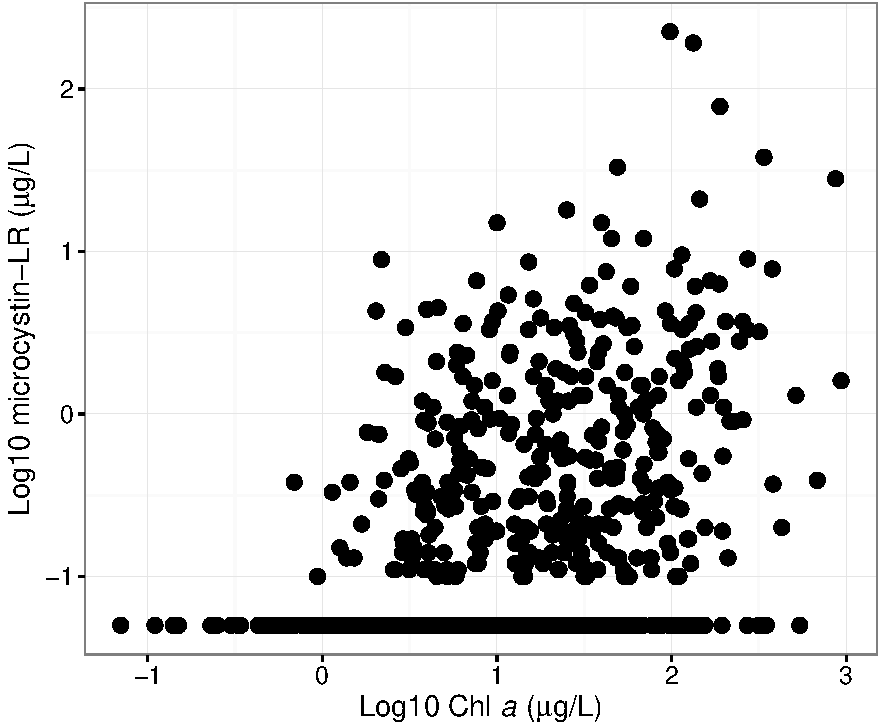
\includegraphics{manuscript_files/figure-latex/chla_micro_scatter-1.pdf}
\caption{Scatterplot showing association betweeen chlorophyll \textit{a}
and microcystin-LR. \label{fig:chla_micro_scatter}}
\end{figure}

\newpage

\begin{verbatim}
## Loading required package: grid
\end{verbatim}

\begin{figure}[htbp]
\centering
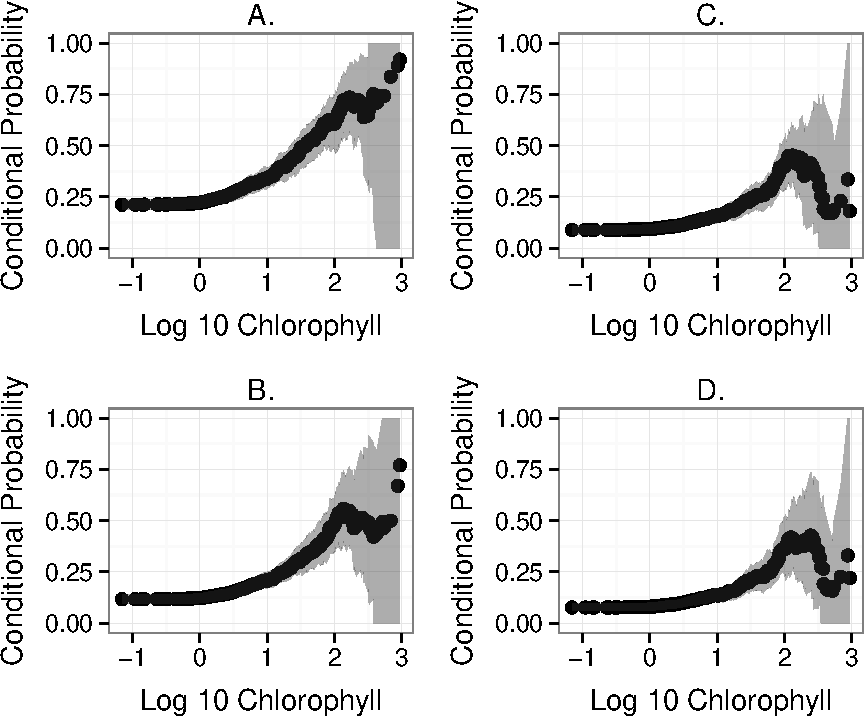
\includegraphics{manuscript_files/figure-latex/epa_child_cp_plot-1.pdf}
\caption{Conditional probability plots showing association between the
probability of exceeding various microcystin-LR (MLR) health advisory
Levels. A.) Plot for U.S. EPA childrens drinking water advisory (0.3
\(\mu\)g/L). B.) Plot for WHO drinking water advisory (1 \(\mu\)g/L).
C.) Plot for U.S. EPA adult drinking water advisory (1.6 \(\mu\)g/L).
D.) Plot for WHO recreational advisory (2 \(\mu\)g/L).
\label{fig:multi_cp_plot}}
\end{figure}

\newpage

\section{Tables}\label{tables}

\begin{longtable}[c]{@{}lll@{}}
\caption{Various suggested microcystin-LR health advisory
concentrations. \label{tab:microcystin_levels}}\tabularnewline
\toprule
Source & Type & Concentration\tabularnewline
\midrule
\endfirsthead
\toprule
Source & Type & Concentration\tabularnewline
\midrule
\endhead
WHO & Drinking & 1 \(\mu\)g/L\tabularnewline
U.S. EPA & Drinking & 0.3 \(\mu\)g/L\tabularnewline
U.S. EPA & Drinking & 1.6 \(\mu\)g/L\tabularnewline
WHO & Recreational & 2-4 \(\mu\)g/L\tabularnewline
WHO & Recreational & 10-20 \(\mu\)g/L\tabularnewline
WHO & Recreational & 20-2000 \(\mu\)g/L\tabularnewline
WHO & Recreational & \textgreater{}2000 \(\mu\)g/L\tabularnewline
\bottomrule
\end{longtable}

\newpage

\begin{longtable}[c]{@{}llrr@{}}
\caption{Chlorophyll \textit{a} concentrations that are associated with
a 50\% probability of exceeding a microcystin-LR health advisory
concentration. \label{tab:mc_chla_table}}\tabularnewline
\toprule
Source & Type & Microcystin & Chlorophyll\tabularnewline
\midrule
\endfirsthead
\toprule
Source & Type & Microcystin & Chlorophyll\tabularnewline
\midrule
\endhead
U.S. EPA & Drinking & 0.3 & 22.56\tabularnewline
WHO & Drinking & 1.0 & 59.40\tabularnewline
U.S. EPA & Drinking & 1.6 & 84.24\tabularnewline
WHO & Recreational & 2.0 & 97.49\tabularnewline
\bottomrule
\end{longtable}

\newpage

\section*{References}\label{references}
\addcontentsline{toc}{section}{References}

Aranda-Rodriguez, R., Z. Jin, J. Harvie, and A. Cabecinha. 2015.
Evaluation of three field test kits to detect microcystins from a public
health perspective. Harmful Algae 42:34--42.

James, R., A. Gregg, A. Dindal, and J. McKernan. 2011. Environmental
technology verification report: Abraxis microcystin test kits. Online
document. Accessed online: June 22.

Jetoo, S., V. I. Grover, and G. Krantzberg. 2015. The toledo drinking
water advisory: Suggested application of the water safety planning
approach. Sustainability 7:9787--9808.

Lee, S., M.-H. Jang, H.-S. Kim, B.-D. Yoon, and H.-M. Oh. 2000.
Variation of microcystin content of microcystis aeruginosa relative to
medium n: P ratio and growth stage. Journal of Applied Microbiology
89:323--329.

McElhiney, J., and L. A. Lawton. 2005. Detection of the cyanobacterial
hepatotoxins microcystins. Toxicology and Applied Pharmacology
203:219--230.

Miller, T. R., L. Beversdorf, S. D. Chaston, and K. D. McMahon. 2013.
Spatiotemporal molecular analysis of cyanobacteria blooms reveals
microcystis-aphanizomenon interactions. PloS one 8:e74933.

Paerl, H. W., and T. G. Otten. 2013. Harmful cyanobacterial blooms:
Causes, consequences, and controls. Microbial ecology 65:995--1010.

Paul, J. F., and W. R. Munns. 2011. Probability surveys, conditional
probability, and ecological risk assessment. Environmental Toxicology
and Chemistry 30:1488--1495.

Rinta-Kanto, J. M., E. A. Konopko, J. M. DeBruyn, R. A. Bourbonniere, G.
L. Boyer, and S. W. Wilhelm. 2009. Lake erie microcystis: Relationship
between microcystin production, dynamics of genotypes and environmental
parameters in a large lake. Harmful Algae 8:665--673.

Zurawell, R. W., H. Chen, J. M. Burke, and E. E. Prepas. 2005.
Hepatotoxic cyanobacteria: A review of the biological importance of
microcystins in freshwater environments. Journal of Toxicology and
Environmental Health, Part B 8:1--37.

\end{document}